% Tópicos previstos na fundamentação teórica: Análises de estratégias de transmissão contínua de dados de monitoramento, estabelecimento de algoritmo de escolha de servidores, balanceadores de carga à nível de aplicação e à nível de rede (dentro e fora do contexto das SDNs), servidores de distribuição de conteúdo e CDNs, uso de memória em servidores de distribuição de conteúdo (\textit{cache} + disco), arquiteturas em servidores de \textit{cache} (e funcionamento básico de \textit{cache} em sistemas de distribuição de conteúdo), estratégias e ferramentas para monitoramento de memória (principal e secundária), estratégias de transmissão contínua de dados de monitoramento de memória, etc.

% Devem ser incluídos os tópicos previstos no plano de TCC

\chapter{Fundamentação Teórica} \label{cap:FundamentacaoTeorica}

Para embasar a proposta central deste trabalho, este capítulo se dedica a revisar os conceitos fundamentais. A exploração detalhada destes pilares teóricos é essencial para contextualizar as decisões metodológicas, o planejamento e a implementação subsequentes e a análise dos resultados, conferindo uma base sólida e coesa ao desenvolvimento da pesquisa.

Serão abordados, inicialmente, os balanceadores de carga, detalhando seu funcionamento e classificações, incluindo abordagens em nível de aplicação e em nível de rede, tanto em contextos tradicionais quanto no âmbito das Redes Definidas por \textit{Software} (SDNs). Em seguida, o foco se voltará aos servidores de distribuição de conteúdo e às Redes de Distribuição de Conteúdo (CDNs), explorando as principais arquiteturas empregadas em seus servidores de \textit{cache} e os modelos de persistência de dados utilizados. Isso incluirá uma análise do funcionamento básico do \textit{cache} nesses sistemas, um componente crucial para a eficiência da entrega de conteúdo.

Posteriormente, serão investigadas as estratégias e ferramentas para o monitoramento de memória, tanto principal (\textit{cache}) quanto secundária (disco), em servidores de distribuição de conteúdo. Este estudo se aprofundará nas técnicas para a transmissão contínua dos dados de monitoramento de memória. A compreensão desses mecanismos é vital, pois o uso de memória é um indicador-chave do desempenho em servidores cujo papel principal é a recuperação e entrega de dados.

A consolidação desses conhecimentos permitirá o estabelecimento conceitual de um algoritmo de escolha de servidores pelo balanceador de carga, fundamentado nos dados de monitoramento de memória, alinhando-se ao objetivo geral de elaborar, implementar e analisar tal algoritmo.

\section{Balanceadores de carga}

Os balanceadores de carga são componentes cruciais na arquitetura de sistemas distribuídos contemporâneos, incluindo ambientes de computação em nuvem e, por extensão, os Sistemas de Distribuição de Conteúdo (CDNs) que são o foco deste trabalho. A função primordial de um balanceador de carga é distribuir de maneira eficiente e inteligente as cargas de trabalho – como requisições de usuários, tráfego de rede ou tarefas de processamento – entre múltiplos recursos computacionais, tipicamente servidores.

A escalabilidade horizontal, caracterizada pela adição de mais computadores a um sistema, tem-se consolidado como uma estratégia preferencial frente à escalabilidade vertical (o aumento de recursos em um computador existente), por sua maior flexibilidade e otimização de custos \cite{scalabilityIssuesInDatabaseSystems}. Como consequência direta dessa abordagem distribuída, os balanceadores de carga assumem um papel crítico, sendo responsáveis por gerenciar a redundância de servidores e direcionar as requisições de forma inteligente, assegurando assim uma utilização eficaz dos recursos.

Esta distribuição estratégica é vital para otimizar a utilização dos recursos disponíveis, maximizar a vazão (\textit{throughput}) de requisições atendidas, minimizar o tempo de resposta para o usuário final e, fundamentalmente, evitar a sobrecarga em qualquer servidor individual. Ao prevenir que um único servidor se torne um ponto de estrangulamento, o balanceamento de carga não apenas aprimora o desempenho geral e a capacidade de escalonamento do sistema, mas também eleva significativamente sua confiabilidade e disponibilidade. Isso ocorre, por exemplo, pela capacidade de detectar falhas em servidores e redirecionar o tráfego para os servidores operantes, garantindo a continuidade do serviço.

A eficácia de um sistema distribuído moderno, portanto, está intrinsecamente ligada à sofisticação e adequação de suas estratégias de balanceamento de carga. Tendo em vista que os balanceadores de carga podem ser concebidos em duas principais categorias - em nível de aplicação e em nível de rede \cite{Pandian2022ICCBI} - nas subseções seguintes serão explorados esses conceitos, diferentes tipos e abordagens de balanceadores de carga, fornecendo a base necessária para a discussão de sua otimização no contexto específico da distribuição de conteúdo baseada em monitoramento de memória.

\subsection{Balanceadores de carga em nível de aplicação}

Os balanceadores de carga em nível de aplicação, também conhecidos como balanceadores de Camada 7 (L7) do modelo OSI ou camada de Aplicação no modelo TCP/IP, operam inspecionando os dados da própria aplicação. Isso significa que eles tomam decisões de roteamento com base em informações contidas no tráfego da aplicação, como cabeçalhos HTTP/HTTPS, \textit{cookies}, tipo de conteúdo (imagens, vídeo, texto) ou qualquer outro dado específico da mensagem.

Diferentemente dos balanceadores de nível de rede, os balanceadores L7 analisam o conteúdo do tráfego, o que permite uma distribuição de carga muito mais granular e inteligente. Por exemplo, um balanceador de carga L7 pode direcionar requisições para servidores diferentes com base na URL solicitada (roteamento baseado em caminho), no tipo de navegador do usuário, ou na linguagem preferida indicada no cabeçalho da requisição. Uma requisição para uma URL de um serviço de arquivos pode ser enviada para um \textit{pool} de servidores otimizado para servir imagens, enquanto requisições para uma \textit{API} podem ser encaminhadas dinamicamente para um \textit{pool} de servidores de aplicação.

Quanto às suas vantagens, os balanceadores L7 permitem decisões de roteamento mais inteligentes e flexíveis, o que resulta em maior eficiência na distribuição de carga, especialmente para aplicações \textit{web} complexas. Adicionalmente, eles oferecem a capacidade de descarregar tarefas computacionalmente intensivas, como a terminação SSL, dos servidores, otimizando o uso de recursos destes.

Por outro lado, os balanceadores de nível de aplicação geralmente consomem mais recursos computacionais (CPU e memória) em comparação com os balanceadores de nível de rede, devido à necessidade de inspecionar e processar o conteúdo detalhado dos pacotes. Este processamento adicional também pode introduzir uma latência ligeiramente maior no encaminhamento das requisições.

Alguns exemplos de balanceadores de carga que atuam na camada de aplicação são:

\begin{enumerate}
    \item \textbf{NGINX:} Amplamente utilizado como servidor \textit{web}, \textit{proxy} reverso e balanceador de carga L7, capaz de rotear tráfego HTTP/HTTPS com base em URLs, cabeçalhos, etc.
    \item \textbf{HAProxy:} Outra solução popular de código aberto que pode operar tanto em L4 (camada de transporte) quanto em L7, oferecendo funcionalidades avançadas de balanceamento HTTP.
    \item \textbf{AWS Application Load Balancer (ALB):} Um serviço gerenciado da \textit{Amazon Web Services} que opera na camada 7, permitindo roteamento avançado de requisições HTTP/HTTPS.
    \item \textbf{Azure Application Gateway:} O balanceador de carga L7 da Microsoft Azure, oferecendo funcionalidades como afinidade de sessão baseada em \textit{cookies}, terminação SSL e \textit{firewall} de aplicação \textit{web} (WAF).
\end{enumerate}

\subsection{Balanceadores de carga em nível de rede}

A introdução das Redes Definidas por \textit{Software} (SDNs) trouxe uma nova perspectiva no contexto de balanceamento de carga, permitindo sua realização em nível de rede sem depender de uma aplicação. A arquitetura SDN ao desacoplar o plano de controle do plano de dados, trouxe uma \textbf{gestão centralizada e programável do encaminhamento de tráfego}, o que é particularmente vantajoso para as estratégias de balanceamento de carga \cite{BelgaumRiyazMusaShahrulnizaAlamMansoorSuudMohd2020}. O controlador SDN, possuindo uma visão global e em tempo real do estado da rede – incluindo topologia, carga dos enlaces e até mesmo estado dos servidores – pode realizar a maior parte das funções que uma aplicação gerenciadora de balanceamento de carga normalmente pode realizar \cite{hamdan2021}. Dessa forma, pode-se conceber que balanceadores de carga de nível de aplicação possuem como principal vantagem a flexibilidade em detrimento do desempenho, enquanto balanceadores de carga de nível de rede possuem como principal vantagem o desempenho mas trazendo como desvantagem uma complexidade e configurabilidade elevadas.

Neste paradigma, a lógica do balanceador de carga pode ser implementada como uma aplicação que reside no topo do controlador SDN. Esta aplicação analisa as informações da rede coletadas pelo controlador e, com base em algoritmos de balanceamento predefinidos ou adaptativos, instrui os dispositivos de encaminhamento (como \textit{switches} \textit{OpenFlow}) sobre como distribuir os fluxos de tráfego entre os servidores disponíveis. Por exemplo, o controlador pode instalar regras nos \textit{switches} para que o tráfego destinado a um determinado endereço IP virtual (VIP) seja distribuído entre um conjunto de endereços IP reais de servidores, utilizando métricas como a menor carga do servidor, menor latência ou maior largura de banda disponível. Esta capacidade de \textbf{programação dinâmica das tabelas de fluxo} nos \textit{switches} permite a implementação de políticas de balanceamento de carga granulares e a rápida adaptação a mudanças na rede ou na carga dos servidores, sem a necessidade de reconfiguração manual de dispositivos individuais.

Uma das principais vantagens do balanceamento de carga em SDNs é a otimização do uso dos recursos da rede e dos servidores. Com a visibilidade global, o controlador SDN pode evitar gargalos e subutilização de recursos de forma mais eficaz \cite{Blial2016}. Além disso, a centralização da inteligência de balanceamento no controlador pode simplificar a infraestrutura de rede, potencialmente reduzindo a necessidade de dispositivos de balanceamento de carga dedicados e caros. A programabilidade também facilita a implementação de algoritmos de balanceamento mais sofisticados que podem considerar múltiplos fatores simultaneamente, realizando a gestão inteligente dos fluxos em nível de rede com base em metadados e estatísticas da rede. A capacidade de resposta a eventos da rede, como falhas de servidores ou congestão de enlaces, é também aprimorada, permitindo um redirecionamento de tráfego mais ágil e eficiente para manter a disponibilidade do serviço.


\section{MPEG-DASH}

O padrão MPEG-DASH é apresentado aqui por ser a tecnologia utilizada na implementação experimental deste trabalho, na qual os servidores fornecem segmentos de vídeo DASH e os clientes são \textit{players} compatíveis com este padrão.

O \textit{streaming} via HTTP se consolidou como prática tecnológica mais aplicada para entrega de conteúdo multimídia graças à popularização do consumo de conteúdo na \textit{web}, à consequente abundância de plataformas \textit{web} e às conexões de banda larga \cite{thang2012adaptive}. Seguindo essa tendência, um novo padrão - \textit{Dynamic Adaptive Streaming over HTTP} (ou simplesmente DASH) - foi desenvolvido de modo a fornecer dinamismo e flexibilidade em diversas situações distintas de conexões de rede. O padrão contrasta com protocolos mais antigos como o RTP (\textit{Real-Time Transport Protocol}), que frequentemente enfrentam problemas com \textit{firewalls} e exigem que os servidores mantenham um estado de sessão para cada cliente. O HTTP oferece uma abordagem sem estado (\textit{stateless}) mais escalável e compatível com a infraestrutura existente \cite{sodagar2011mpegdash}. Aproveitando essa base, foi desenvolvido o padrão \textit{Dynamic Adaptive Streaming over HTTP} (MPEG-DASH), com o objetivo de criar uma solução interoperável para o \textit{streaming} adaptativo, unificando um mercado anteriormente fragmentado por soluções proprietárias \cite{sodagar2011mpegdash}.

A arquitetura do MPEG-DASH é fundamentalmente orientada ao cliente. O servidor de conteúdo tem a função de preparar e disponibilizar o material, mas toda a inteligência da sessão de \textit{streaming} reside no cliente \cite{stockhammer2011dynamic}. Isso significa que o servidor não precisa gerenciar o estado da conexão, permitindo que servidores HTTP e redes de distribuição de conteúdo (CDNs) convencionais sejam utilizados para a entrega em larga escala de forma eficiente \cite{stockhammer2011dynamic}. A operação do padrão se baseia em dois componentes principais:

\begin{enumerate}
    \item \textbf{Media Presentation Description (MPD):} É um arquivo de manifesto, geralmente em formato XML, que descreve a estrutura e as diferentes versões do conteúdo multimídia disponíveis \cite{sodagar2011mpegdash}. O MPD organiza o conteúdo hierarquicamente em Períodos (\textit{Periods}), que representam intervalos de tempo; Conjuntos de Adaptação (\textit{Adaptation Sets}), que agrupam alternativas de um mesmo componente de mídia (como diferentes idiomas de áudio ou ângulos de câmera); e Representações (\textit{Representations}), que são as diferentes versões de um mesmo fluxo, codificadas com distintas taxas de \textit{bits}, resoluções ou qualidades \cite{sodagar2011mpegdash}. O MPD contém os metadados essenciais, incluindo as URLs para acessar cada parte do conteúdo.

    \item \textbf{Segmentos:} O conteúdo de mídia em si é dividido em pequenos blocos sequenciais chamados segmentos \cite{sodagar2011mpegdash}. Cada representação possui sua própria sequência de segmentos, que são requisitados individualmente pelo cliente através de requisições HTTP GET padrão \cite{stockhammer2011dynamic}. Por serem arquivos independentes acessados via HTTP, os segmentos são facilmente armazenáveis em \textit{cache} por \textit{proxies} e CDNs, o que é um dos pilares da escalabilidade do DASH.
\end{enumerate}

O fluxo de trabalho típico de uma sessão DASH começa com o cliente requisitando e analisando o arquivo MPD \cite{sodagar2011mpegdash}. Com base nas informações do manifesto, nas condições atuais da rede (como a largura de banda estimada), nas capacidades do dispositivo (como resolução de tela) e nas preferências do usuário, a lógica de controle do cliente (conhecida como \textit{decision engine} ou \textit{control heuristics}) seleciona a representação mais apropriada para iniciar a reprodução \cite{thang2012adaptive}. É importante notar que essa lógica de decisão e adaptação não é padronizada pelo MPEG-DASH, o que confere flexibilidade aos desenvolvedores de clientes \cite{sodagar2011mpegdash}. Após o início da reprodução, o cliente continua a requisitar os segmentos sequencialmente, monitorando o desempenho da rede e, se necessário, trocando para uma representação de maior ou menor qualidade para garantir uma reprodução contínua e com a melhor Qualidade de Experiência, do inglês \textit{Quality of Experience}, (QoE) para o usuário possível.

\subsection{\textit{Content Steering}}

O \textit{Content Steering} (direcionamento de conteúdo) é um mecanismo que estende a capacidade de adaptação do cliente para além da simples seleção da qualidade do fluxo de mídia. Em vez de apenas decidir o que buscar (qual representação), o \textit{Content Steering} permite ao cliente decidir de onde buscar o conteúdo, ou seja, de qual servidor ou CDN obter os segmentos \cite{sodagar2011mpegdash}.

O padrão MPEG-DASH facilita essa funcionalidade diretamente no \textit{Media Presentation Description} (MPD) através da especificação de múltiplas URLs base (\textit{BaseURL}). O MPD pode listar vários endereços para o mesmo conjunto de segmentos, onde cada URL pode apontar para um servidor espelho, um \textit{data center} geograficamente distinto ou até mesmo uma CDN completamente diferente \cite{sodagar2011mpegdash}.

A responsabilidade de escolher qual URL base utilizar recai inteiramente sobre a lógica de controle do cliente, pois o padrão apenas fornece o mecanismo, mas não dita a política de seleção \cite{sodagar2011mpegdash}. Um cliente pode implementar estratégias de direcionamento para:
\begin{itemize}
    \item \textbf{Otimizar o desempenho:} O cliente pode medir a latência ou a vazão para cada uma das URLs base disponíveis e selecionar aquela que oferece o melhor desempenho em um dado momento.
    \item \textbf{Aumentar a confiabilidade:} Caso a requisição para um segmento a partir de uma URL base falhe ou se torne excessivamente lenta, o cliente pode dinamicamente tentar buscar o mesmo segmento (ou os segmentos subsequentes) a partir de uma URL base alternativa, criando um mecanismo de \textit{failover} no nível da aplicação.
    \item \textbf{Balancear a carga:} Em cenários mais avançados, o cliente poderia distribuir suas requisições entre múltiplas fontes de conteúdo para maximizar a largura de banda disponível e evitar sobrecarregar um único servidor ou rota de rede \cite{sodagar2011mpegdash}.
\end{itemize}

Dessa forma, o \textit{Content Steering} transforma o cliente DASH em um participante ativo no balanceamento de carga e na otimização da entrega, tornando o padrão altamente resiliente e adaptável a implantações de grande escala que envolvem múltiplas CDNs e infraestruturas de servidores complexas.

\section{Servidores de distribuição de conteúdo e CDNs}

Esta seção estabelece o contexto de aplicação do algoritmo proposto. Como os servidores de distribuição de conteúdo têm como função principal recuperar e entregar dados, o uso de memória é um indicador-chave de desempenho, justificando sua escolha como métrica de balanceamento.

As Redes de Entrega de Conteúdo (popularmente conhecidas como \textit{Content Delivery Networks} ou CDNs) são uma parte crítica da infraestrutura da Internet, criada para distribuir conteúdo de forma rápida, confiável e eficiente. Elas atingem esse objetivo por meio da distribuição redundante de conteúdo em vários servidores geograficamente dispersos. Quando um usuário realiza uma requisição para um conteúdo por meio de um serviço \textit{web}, a requisição é encaminhada dinamicamente para o servidor mais próximo do usuário em vez de ser enviada para o servidor de origem do conteúdo. Essa é uma prática simples que reduz a latência, minimiza a perda de pacotes (por diminuir o número de saltos) e remove a sobrecarga de servidores que possuem o conteúdo original, resultando em uma QoE mais elevada.

É interessante notar também que as Redes de Entrega de Conteúdo, apesar de serem conjuntos de dispositivos computacionais interconectados assim como as redes de computadores tradicionais, não são necessariamente um subconjunto dessas redes no contexto conceitual. Em vez disso, são sistemas distribuídos de computadores, geralmente administrados em nível de aplicação por uma organização privada. Em outras palavras, são grupos de computadores que se comunicam de forma padronizada para cumprir com o objetivo de entregar conteúdo para os usuários finais, mas que não estão no mesmo nível de abstração conceitual das redes de computadores. Dessa forma, as CDNs são, na verdade, arquiteturas de aplicação altamente complexas e flexíveis e que, por extensão, estão localizadas no topo da pilha de abstração de camadas de rede - a camada de aplicação.

Nesse sentido, considerando que o princípio central das CDNs é aumentar a taxa de transmissão e diminuir a latência por meio da aproximação física do conteúdo aos usuários, os seus mecanismos-chave são:

\begin{enumerate}
    \item{\textbf{Arquitetura}}: Predominantemente, as CDNs se organizam em duas camadas principais de servidores: \textbf{Os servidores de origem} que detém o conteúdo original e os servidores de borda que possuem cópias redundantes dos conteúdos e são posicionados estrategicamente mais próximos dos usuários finais. Esses servidores de borda são organizados em \textit{Points of Presence} (PoPs), \textit{Data Centers} organizados com o intuito de dispor servidores de borda para as CDNs. 
    \item{\textbf{\textit{Cache}}}: As CDNs possuem vários servidores de borda localizados em regiões geográficas distribuídas. Quando um usuário realiza uma requisição para o conteúdo em questão, a CDN responde com o conteúdo do servidor localizado no PoP mais próximo, significativamente reduzindo a distância física sobre qual a requisição precisa trafegar. Esse funcionamento básico reduz a latência e aumenta a taxa de transmissão de dados, ainda sendo efetivo para a Internet sob o ponto de vista de ecossistema, uma vez que há menos requisições geograficamente dispersas evitando sobrecarregar a rede global.
    \item{\textbf{Roteamento}}: As CDNs se beneficiam de várias técnicas para determinar o melhor PoP para lidar com uma requisição do usuário. Uma das técnicas para realizar esse processo é a utilização de roteamento baseado em DNS, no qual o sistema DNS da CDN direciona o usuário para o endereço de IP do servidor mais apropriado baseado na localização geográfica.
    \item{\textbf{Balanceamento de carga}}: As redes de entrega de conteúdo distribuem requisições dos usuários para evitar que quaisquer servidores de um PoP se sobrecarreguem. Conforme mencionado, o principal fator para distribuição de requisições entre servidores é a localização geográfica. No entanto, outras técnicas mais avançadas também são empregadas, como \textit{anycast} \cite{Preston2021Finding}, na qual os servidores de borda anunciam possuir o mesmo endereço IP através de um roteador BGP e, naturalmente, o servidor geograficamente mais próximo da requisição efetivamente recebe e a processa.
\end{enumerate}

Para os servidores de borda das CDNs, que estão dispostos em larga escala, se configurados apenas com as tarefas de entrega de conteúdo estático pré-processado (como é o caso do \textit{MPEG-DASH}), é correto dizer que eles teriam menos tarefas intensivas de processo específicas de conteúdo no momento da entrega em comparação com, por exemplo, a transcodificação de vídeo instantânea ou a geração de conteúdo dinâmico durante o tratamento de cada requisição. Nesse sentido, faz sentido conceber que os recursos computacionais mais utilizados nesse caso são os recursos de armazenamento - tanto em memória principal quanto em memória secundária.

\subsection{Funcionamento de \textit{cache} em redes de entrega de conteúdo}

Na complexidade intrínseca às CDNs, se encontram múltiplas camadas de \textit{caching} de modo a cumprir com o propósito de evitar tráfego em amplas distâncias. Conforme a Figura \ref{fig:cdn-caching}, é possível conceber pelo menos três níveis nas arquiteturas tradicionais de CDNs \cite{cdnStatusAndTrends2003}:

\begin{enumerate}
    \item{\textbf{Acesso direto ao \textit{Proxy}}}: Na primeira iteração de uma requisição que passa por uma CDN, é realizada uma verificação nos servidores de \textit{proxy} dos provedores de rede (ISPs). Os servidores \textit{proxy} são basicamente computadores (físicos ou virtuais) dispostos diretamente nas infraestruturas dos provedores de serviço, mantidos para armazenar conteúdo frequentemente acessado pelos usuários e até mesmo evitar sobrecarga nos servidores de borda das CDNs.
    \item{\textbf{Acesso iterativo aos servidores de borda da CDN}}: Em segundo plano, são realizadas tentativas sucessivas de acesso ao conteúdo requisitado através dos servidores de borda da CDN, um por vez. Ao encontrar o conteúdo em questão, ele pode ser armazenado em \textit{cache} nos servidores nos quais o conteúdo não foi encontrado.
    \item{\textbf{\textit{Peering} de CDNs}}: Em algumas CDNs específicas, maiores e mais complexas, é possível que seja realizada uma configuração de colaboração (\textit{peering}) que faz com que CDNs possam buscar por conteúdo em outras CDNs, aumentando ainda mais a eficiência. 
\end{enumerate}

É válido conceber que o funcionamento geral de uma CDN consiste na disposição e organização de servidores (físicos e virtuais) de modo a minimizar a distância percorrida por pacotes de requisições na Internet. Além disso, sabe-se que a ferramenta tecnológica mais utilizada para escolher dinamicamente o servidor conforme o conteúdo requisitado e distâncias geográficas é o roteamento dinâmico de DNS, considerada a técnica mais popular no contexto das CDNs \cite{dnsBasedCdnsEvolutionAndChallenges2018}.

\begin{figure}[htbp]
    \caption{Estrutura básica de uma CDN.}
    \centering
    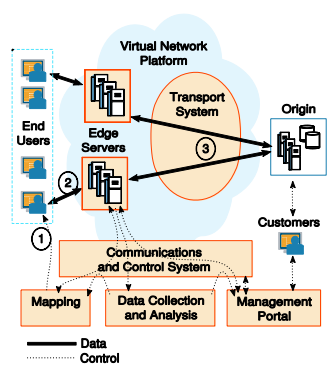
\includegraphics[width=0.7\linewidth]{./Textuais/2-FundamentacaoTeorica/cdn-diagram.png}
    \text{Fonte: Adaptado de \cite{akamaiNetwork2010}}
    \label{fig:cdn-structure}
\end{figure}

\begin{figure}[htbp]
    \caption{Fluxo detalhado das múltiplas camadas de \textit{caching} em CDNs.}
    \centering
    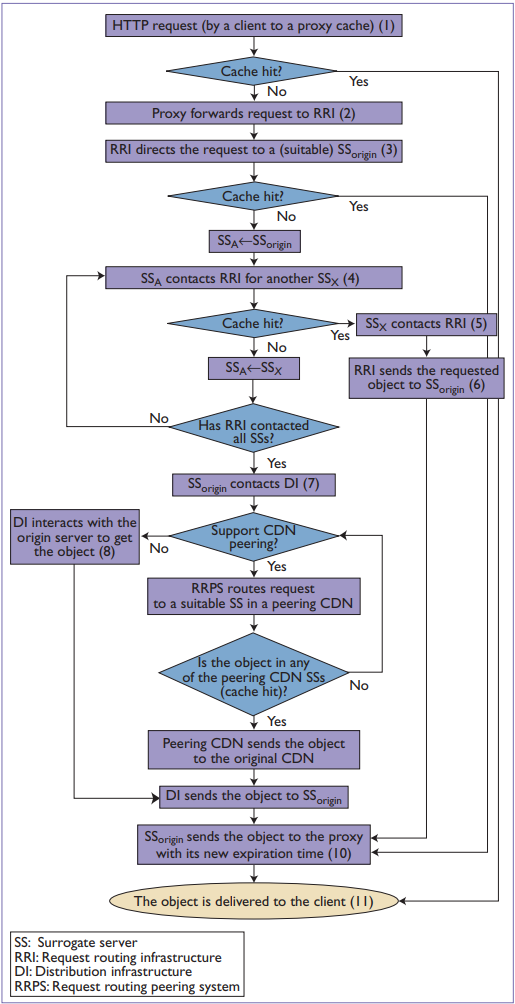
\includegraphics[width=0.7\linewidth]{./Textuais/2-FundamentacaoTeorica/cdn-caching-structure.png}
    \text{Fonte: Adaptado de \cite{cdnStatusAndTrends2003}}
    \label{fig:cdn-caching}
\end{figure}

\section{Monitoramento de memória}

Esta seção é central para o trabalho, pois o algoritmo proposto utiliza exclusivamente métricas de memória principal e secundária como parâmetros de decisão para o balanceamento de carga.

Com a emergente necessidade de modernizar e escalar sistemas nos mais diversos setores da indústria, por consequência, emergiu também, no contexto tecnológico, a necessidade da disponibilização de recursos computacionais sob demanda de modo mais flexível possível. Esse fenômeno resultou no paradigma de disponibilização de recursos computacionais de forma mais abstrata e encapsulada, conhecido como Computação em Nuvem (\textit{Cloud Computing}) \cite{boss2007cloud}. Junto com a aplicação do novo paradigma, também se fez necessária a evolução sistemática dos processos de monitoramento de recursos computacionais e de rede, como vazão de dados, latência, processamento da CPU, uso de memória principal e secundária, dentre outros.

\subsection{APIs fornecidas pelos principais sistemas operacionais}

A principal e mais utilizada maneira de se obter a métrica do consumo de memória é por meio de APIs disponibilizadas pelos Sistemas Operacionais. A maioria dos \textit{Kernels}, durante o gerenciamento de memória e de disco relacionados aos processos gerenciados, possui instruções para armazenar e recuperar informações, atualizadas constantemente, a respeito do consumo de memória e de disco. Embora a disposição dessas informações seja diferente de sistema para sistema, a maior parte deles disponibiliza uma API para que aplicações no espaço do usuário (\textit{user-space}) consigam obter essa informação.

Para o sistema operacional \textit{Linux}, por exemplo, a interface primária para monitoramento é o diretório virtual \texttt{/proc/meminfo}. Através deste diretório, o SO fornece uma análise detalhada do uso da RAM (\textit{Random Access Memory} - ou Memória Principal) \cite{linux_procfs_doc}. Além disso, o SO fornece informações detalhadas sobre estatísticas de leitura para cada bloco no disco (memória secundária) por meio do diretório \texttt{/proc/diskstats} \cite{linux_iostats_doc}. Outros sistemas operacionais possuem seus próprios métodos e APIs para disponibilizar essas informações. Enquanto o \textit{macOS} utiliza subsistemas \cite{macos_iokit_doc} \cite{macos_virtmem_doc},o \textit{Windows} possui uma API bem definida baseada em requisições denominada \textit{Performance Counters}, que sistematicamente disponibiliza essas informações \cite{windows_disk_counters} \cite{windows_mem_counters}.

\subsection{Aplicações}

Com base no princípio anterior, existem várias soluções em nível de aplicação que referenciam o sistema operacional de forma dinâmica para dispor, transportar e processar essas informações de monitoramento de forma sistemática. Alguns exemplos são: o sistema \textit{Tivoli® Monitoring} da IBM \cite{boss2007cloud}, o clássico \textit{Task Manager} do \textit{Windows}, as soluções de linha de comando \texttt{top}, \texttt{htop} e \texttt{free} do \textit{Linux}, dentre outras aplicações que podem funcionar tanto de forma isolada quanto distribuída.
 
\section{Interpretação de dados desatualizados}

Esta seção é crítica, pois o algoritmo proposto depende de informações de memória coletadas periodicamente, criando um intervalo entre a coleta e o uso durante o qual o estado dos servidores pode mudar. O trabalho "\textit{Interpreting Stale Load Information}" \cite{interpretingStaleLoadInformation2000} fornece a base teórica para o algoritmo implementado, através da adaptação do método \textit{Basic LI}.

No contexto de balanceamento de carga, é fato que a estratégia de direcionamento da carga para a máquina com menos sobrecarga pode ter desempenho ruim se a informação de carga dos servidores estiver relativamente desatualizada \cite{adaptiveLoadSharing1986, analysisDelaysLoadSharing1989, howUsefulIsLoadInformation2000, loadDistributingInLocallyDistributedSystems1993}. Nesse sentido, sistemas de balanceamento de carga que possuem como estratégia a escolha de servidores pouco sobrecarregados que não tratam devidamente a desatualização da informação de carga dos servidores podem produzir o efeito contrário ao desejado, efetivamente sobrecarregando as máquinas que processam requisições.

A falta de tratamento devido a dados desatualizados pode causar um fenômeno no qual máquinas que aparentam estar subutilizadas rapidamente se tornam sobrecarregadas, uma vez que, durante a defasagem da propagação da informação, todos os clientes enviam suas requisições para as mesmas máquinas, que por sua vez ficam sobrecarregadas até que uma nova informação de carga seja propagada pelo sistema. Para combater esse problema, algumas abordagens comuns incluem o uso de algoritmos de seleção aleatória ou \textit{Round-Robin}, que ignoram completamente os dados de carga, ou o uso de um subconjunto aleatório de servidores para a tomada de decisão.

Por outro lado, se for imprescindível que os dados de sobrecarga de um ou mais recursos computacionais dos servidores gerenciados sejam considerados variáveis utilizadas pela estratégia de balanceamento de carga, existem algumas estratégias para resolver o problema da desatualização dos dados. O trabalho "\textit{Interpreting Stale Load Information}" \cite{interpretingStaleLoadInformation2000} desenvolve estratégias que interpretam a informação de carga com base em sua idade em vez de arriscar um desempenho extremamente baixo ou ignorar a oportunidade de usar essa informação para otimizar o sistema.

\section{Virtualização de redes para simulação de cenários}

A virtualização de redes é apresentada aqui por ser a tecnologia utilizada na implementação experimental, onde toda a infraestrutura foi implementada em contêineres Docker, permitindo a simulação de múltiplos servidores em uma única máquina física.

A virtualização de redes surgiu como uma abordagem para flexibilização da adição de novas tecnologias na arquitetura da Internet, extremamente necessária em um cenário no qual a introdução de novas tecnologias radicalmente diferentes se tornou praticamente impossível devido à necessidade de consenso entre múltiplos \textit{stakeholders} com objetivos conflitantes. Esse conceito propõe permitir a coexistência de múltiplas arquiteturas de rede heterogêneas sobre uma infraestrutura física compartilhada, promovendo assim a inovação e o desenvolvimento de aplicações diversificadas \cite{aSurveyOfNetworkVirtualization2010}.

Uma rede virtual é essencialmente uma coleção de nós e links virtuais, representando um subconjunto dos recursos da rede física subjacente. A ideia fundamental é separar as responsabilidades dos tradicionais Provedores de Serviço de Internet (ISPs) em duas novas entidades: os Provedores de Infraestrutura (InPs), que gerenciam os recursos físicos, e os Provedores de Serviço (SPs), que criam redes virtuais ao agregar recursos de múltiplos InPs para oferecer serviços de ponta a ponta \cite{aSurveyOfNetworkVirtualization2010}. Essa separação cria um ambiente dinâmico que facilita a implantação de arquiteturas heterogêneas coexistentes, superando as limitações da Internet atual. A virtualização visa atingir objetivos de \textit{design} como flexibilidade, heterogeneidade, gerenciabilidade, isolamento e programabilidade.

\subsection{Virtualização baseada em contêineres \textit{Linux}}

Enquanto a virtualização tradicional, por meio de Máquinas Virtuais (VMs), emula uma plataforma de \textit{hardware} completa, exigindo um sistema operacional convidado (\textit{GuestOS}) completo e um \textit{software} de monitoramento (VMM ou \textit{hypervisor}), a virtualização em nível de sistema operacional, ou baseada em contêineres, adota uma abordagem mais leve. Nesta técnica, o \textit{kernel} do sistema operacional hospedeiro é modificado para suportar múltiplas instâncias isoladas do espaço de usuário (os contêineres). Como os programas dentro dos contêineres utilizam diretamente a API do sistema hospedeiro, o \textit{overhead} de virtualização é mínimo, uma vez que não há necessidade de emulação de \textit{hardware}. Essa eficiência torna os contêineres, como o LXC (\textit{Linux} contêineres), uma tecnologia chave para plataformas de emulação, permitindo que múltiplos "\textit{netboxes}" (redes virtuais encapsuladas) executem de forma concorrente e autônoma em um único PC, com recursos computacionais privados e isolados.

Para construir redes virtuais, a abstração das interfaces de rede é fundamental. Em um ambiente de contêineres, isso é alcançado pela criação de interfaces de rede virtuais (como pares \textit{Virtual Ethernet} ou VETH) que operam como túneis. O núcleo de uma "\textit{netbox}" é um motor de simulação (como o NS-3) executando dentro de um contêiner, onde os nós da rede simulada são equipados com interfaces do tipo \textit{Ethernet}. Essas interfaces são então ligadas às interfaces virtuais do contêiner. Os contêineres podem ser interligados por meio de \textit{bridges} de \textit{software} que rodam no sistema hospedeiro ou conectados diretamente a placas de rede físicas (NICs), permitindo a comunicação com entidades externas ou outras \textit{netboxes}. Essa arquitetura permite que a cascata de múltiplas \textit{netboxes} sintetize as diferentes seções de uma rede heterogênea complexa, com cada \textit{netbox} emulando as características de uma rede específica de forma exclusiva e isolada.

\section{Trabalhos relacionados}

O sistema NGINX é amplamente utilizado como servidor \textit{Web}, \textit{proxy} reverso e balanceador de carga para lidar com aplicações de alta concorrência. Seus algoritmos nativos de balanceamento, como \textit{Weighted Round-Robin}, \textit{Least Connections} e \textit{IP hash}, são as estratégias mais comuns. A abordagem \textit{IP hash}, por exemplo, foi projetada para direcionar requisições de um mesmo cliente para o mesmo servidor, mantendo a continuidade da sessão.  Contudo, a função de \textit{hash} nativa é considerada muito simples, o que leva a uma alta probabilidade de "colisões de \textit{hash}".  Essas colisões resultam em uma distribuição de carga não uniforme, fazendo com que alguns servidores fiquem sobrecarregados enquanto outros permanecem subutilizados \cite{nginxAlgorithmsEvaluationYuhong2022}. Essa limitação evidencia que, embora os balanceadores de carga baseados no NGINX sejam eficientes em distribuir o tráfego de modo geral, não há uma estratégia que monitore o uso de memória em tempo real para ajudar na tomada de decisões dinâmicas, sobretudo no contexto de distribuição de conteúdo, cenário no qual a recuperação de arquivos em memória é predominante. Isso pode resultar em sobrecarga nos servidores de \textit{cache}, especialmente em cenários de alto tráfego, onde a memória é um recurso crítico. Portanto, a adição de uma camada de monitoramento de memória pode aprimorar a inteligência do balanceador de carga, permitindo uma alocação de tráfego que considere o estado real dos recursos do servidor, em vez de depender apenas de heurísticas de distribuição.

O \textit{HAProxy} \cite{haproxy} é um \textit{software} de código aberto que fornece balanceamento de carga e \textit{proxy} reverso para aplicações baseadas em TCP/IP e HTTP. Embora seja reconhecido por sua eficiência e baixo uso de memória, não há indicações de que utilize monitoramento de memória em tempo real para otimizar a distribuição de tráfego. Integrar tal funcionalidade poderia aprimorar a alocação de recursos e prevenir sobrecargas nos servidores de \textit{cache}.

No contexto da poderosa e moderna prática de conteinerização de servidores, o \textit{Docker} é uma plataforma de código aberto disponibilizada especificamente para esse propósito. O \textit{Docker Swarm}, mecanismo interno da plataforma, realiza a orquestração sistemática de contêineres em sistemas complexos e computacionalmente descentralizados. Embora a ferramenta possua um mecanismo interno de balanceamento de carga, o roteamento é feito utilizando técnicas simples como \textit{Round-Robin} e distribuição aleatória para realizar o roteamento distribuído de requisições para os servidores em contêineres. Em 2018, foi realizado um experimento utilizando essas ferramentas de modo a introduzir a influência do consumo de memória nos servidores e, consequentemente, aumentar a eficiência do balanceador de carga \cite{dockerswarmmemory2018}. No entanto, a pesquisa não só teve foco exclusivamente voltado às especificidades da ferramenta \textit{Docker}, mas também não envolveu nenhuma análise no contexto de servidores de distribuição de conteúdo.

Também foram elaborados vários algoritmos que tornam o balanceamento de carga dinâmico (\textit{Dynamic Load Balancing}). Um deles \cite{novelWeightAssignmentLoadBalancingAlgorithmForCloudApps2023} teve foco na determinação e uso de métricas cuidadosamente selecionadas para recursos computacionais dos servidores de destino: Número de \textit{threads}, tamanho do \textit{buffer} de rede, consumo de \textit{CPU}, consumo de memória e largura de banda. O objetivo do trabalho é propor uma nova técnica para a resolução do problema causado pelo fenômeno recorrente na \textit{web} chamado de \textit{Flash Crowds}, caracterizado pelo aumento abrupto de requisições de clientes em serviços \textit{web}. O trabalho trata de aplicações \textit{cloud} no geral, não tendo especificidade voltada a servidores de distribuição de conteúdo.

Uma revisão \cite{webServerPerformanceImprovement2021Review} foi realizada de modo a obter um retrato do panorama geral das técnicas mais utilizadas para o balanceamento de carga. Após a apresentação dos algoritmos, uma comparação sistemática foi realizada entre eles e um dos critérios de comparação foi a parametrização utilizada por cada algoritmo. Quase todos os algoritmos apresentados pela revisão são dinâmicos e utilizam mais de um parâmetro de configuração. Do total de 15 algoritmos apresentados, 11 usam o tempo de resposta da requisição como parâmetro, 9 utilizam a vazão de dados, 6 utilizam consumo de memória nos servidores, 6 utilizam o consumo de disco, 5 usam o consumo de recursos computacionais em geral na unidade do servidor, 4 usam especificamente o consumo de \textit{CPU}, 4 usam como parâmetro a duração média das requisições (que se diferencia do tempo de resposta, visto que este é monitorado individualmente por requisições de teste que não refletem a carga verdadeira), 2 usam técnicas simples como \textit{Round-Robin} e distribuição aleatória, 1 usa a taxa de falha de requisições e 1 usa o número de conexões simultaneamente ativas. Dessa forma, percebe-se que, na revisão, não há nenhum algoritmo que possivelmente fundamentaria a criação de uma arquitetura de balanceamento de carga especificamente voltada para servidores de distribuição de conteúdo, tendo como base exclusivamente o monitoramento de memória em servidores.

No trabalho "\textit{Dynamic Load Balancing for Efficient Video Streaming Service}" \cite{dynamicLoadBalancingForEfficientVideoStreamingService2015}, é abordado o desequilíbrio de carga em servidores de \textit{streaming} causado pela concentração de requisições em conteúdos populares. A estratégia proposta é um sistema de gerenciamento de conteúdo dinâmico, denominado iSCON, que monitora os servidores em tempo real e redistribui a carga por meio da replicação de conteúdos populares em servidores com menor tráfego. A abordagem dos autores se concentra exclusivamente na largura de banda de transmissão como o principal indicador de carga; o algoritmo de balanceamento é acionado quando a largura de banda de um servidor excede um limiar predefinido. Embora as especificações dos servidores, incluindo a memória \textit{RAM}, sejam detalhadas, o monitoramento do uso de memória não é considerado um parâmetro para as decisões de balanceamento de carga. O foco permanece na equalização do tráfego de rede, deixando uma lacuna na otimização de cenários onde a pressão sobre a memória, e não apenas a saturação da largura de banda, pode se tornar o gargalo para o desempenho do sistema de distribuição de conteúdo.

No trabalho "\textit{Data Allocation and Dynamic Load Balancing for Distributed Video Storage Server}", \cite{dataAllocationAndDynamicLoadBalancingForDistributedVideoStorageServer1999} propõem uma solução de duas fases para aumentar a disponibilidade em um \textit{cluster} de servidores de vídeo distribuídos. A primeira fase consiste em um esquema de alocação inicial de dados que distribui réplicas de vídeo pelos servidores com base em probabilidades de acesso esperadas, a fim de alcançar um balanceamento de carga estático. A segunda fase é uma estratégia de balanceamento de carga dinâmica chamada "\textit{load shifting}" (deslocamento de carga), na qual uma requisição bloqueada em um servidor sobrecarregado pode ser admitida ao se migrar uma ou mais requisições já em andamento daquele servidor para outros nós no \textit{cluster}, potencialmente em uma reação em cadeia. O acionamento deste mecanismo dinâmico é baseado em limiares predefinidos que comparam a carga de um servidor, medida pelo número de \textit{streams} ativas ($P_{i,j}$), com a carga de seus vizinhos ou com sua capacidade máxima de serviço ($A_{max}$). O conceito de "carga" é, portanto, uma função do número de \textit{streams} ativas em relação à capacidade máxima do servidor, sem considerar o estado de recursos de mais baixo nível, como o uso de memória ou \textit{CPU}. Esta abstração é eficaz para balancear o número de requisições, mas não endereça potenciais gargalos de desempenho que podem surgir do esgotamento da memória do sistema, especialmente em servidores que realizam \textit{cache} intensivo de dados de vídeo, um problema que o presente estudo visa investigar.

\section{Considerações}

Este capítulo apresentou os fundamentos teóricos essenciais para o desenvolvimento da proposta deste trabalho. A exploração dos balanceadores de carga, tanto em nível de aplicação quanto em nível de rede, estabeleceu a base conceitual necessária para compreender as diferentes abordagens arquiteturais disponíveis e justificar a escolha pela implementação em nível de aplicação.

O estudo do padrão MPEG-DASH e do funcionamento das CDNs forneceu o contexto de aplicação específico, evidenciando que servidores de distribuição de conteúdo dependem intensivamente de operações de memória, tanto principal quanto secundária. Esta característica operacional fundamenta a escolha do monitoramento de memória como métrica central para o algoritmo de balanceamento proposto.

A revisão das técnicas de monitoramento de memória e das estratégias para interpretação de dados desatualizados forneceu os mecanismos técnicos e teóricos necessários para a implementação prática. Especificamente, o trabalho "\textit{Interpreting Stale Load Information}" oferece a base algorítmica para lidar com a defasagem temporal inerente ao processo de monitoramento distribuído.

A análise dos trabalhos relacionados demonstrou que, embora existam diversas abordagens de balanceamento de carga dinâmico, não há trabalhos que se concentrem exclusivamente no monitoramento de memória para balanceamento em servidores de distribuição de conteúdo, estabelecendo assim a originalidade e relevância da proposta apresentada.

Por fim, a exploração da virtualização de redes, especialmente baseada em contêineres, justificou as escolhas arquiteturais para a implementação experimental, permitindo a realização de experimentos controlados em um ambiente isolado.
